\subsection{Out of Place Measurement}

\subsubsection{Metric description}

This measure determines how far out of place an N-gram in one profile is from its place in the other profile. It allows us to consider the change in the importance of common word of the two corpses. The rank of the n-gram is its order by its frequency. If a word appears or disappear it has a maximum value rank. Otherwise, we sum to the metric the change of rank of the n-gram. The process of computation can be concluded as follows:

\begin{eqnarray}\label{outofplace}
	D(i, j) = \sum_{x \in D_i \bigcap x \in D_j} |R_x^i - R_x^j| + 
			\max_{x \in D_i \bigcap x \in D_j}(R_x^i - R_x^j) (\sum_{x \in (D_i - D_j)} 1 + \sum_{x \in (D_j - D_i)} 1)
\end{eqnarray}

\subsubsection{Computation of \emph{Out of Place} measurement}

In the experiment, the \emph{Out of Place} measurement is divided to two methods (i.e., whether to use the unmatched word's frequency. We also computed the \emph{Out of Place} with the non-corrected corpus and the OCR-corrected corpus to see the impact of OCR correction. The figures illustrated below explain the performance of \emph{Out of Place} under different conditions in the dataset of 1-gram. For the experiment on 2-gram and 3-gram, they have similar performance to 1-gram, and details are omitted.

\begin{figure}[H]
    \begin{minipage}[b]{0.48\linewidth}
        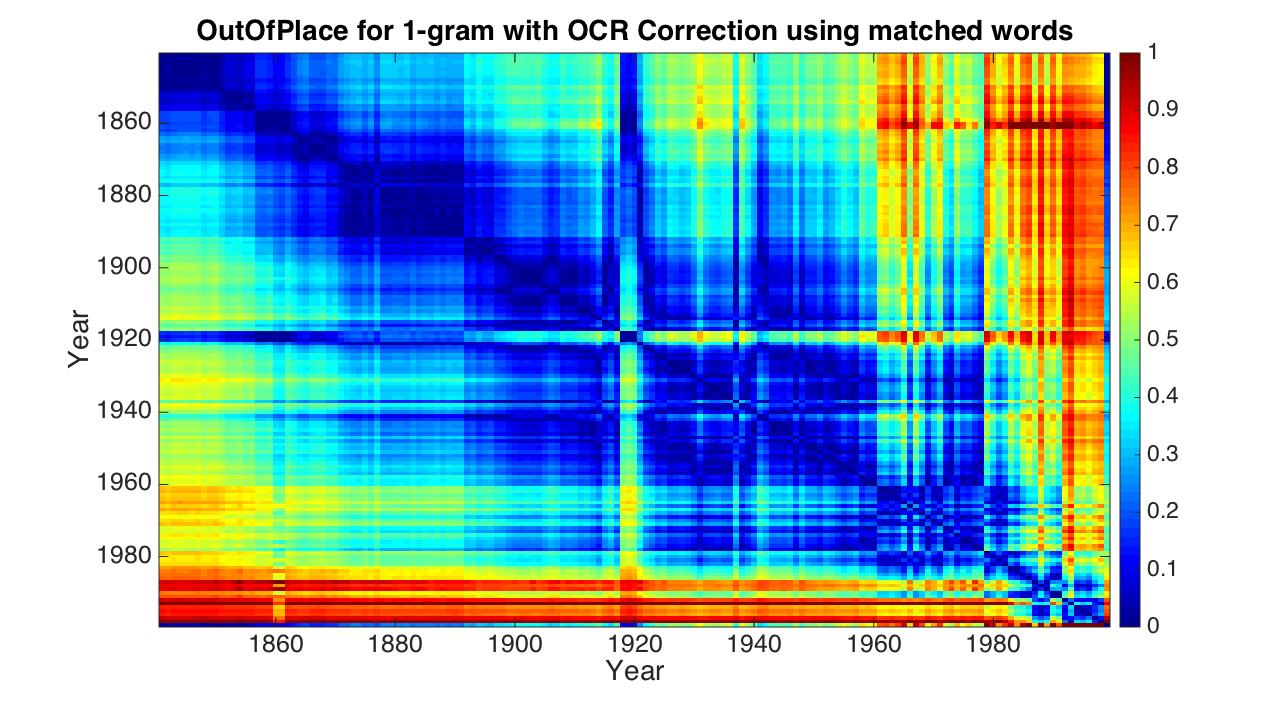
\includegraphics[scale=0.15]{Pictures/outofplace/outofplace_1-gram_correctedOCR_matched_words.jpg}
        \caption{Outofplace for 1-gram with OCR correction using matched words}
        \label{outofplace_1_match_correct}
    \end{minipage}\hfill
    \begin{minipage}[b]{0.5\linewidth}
        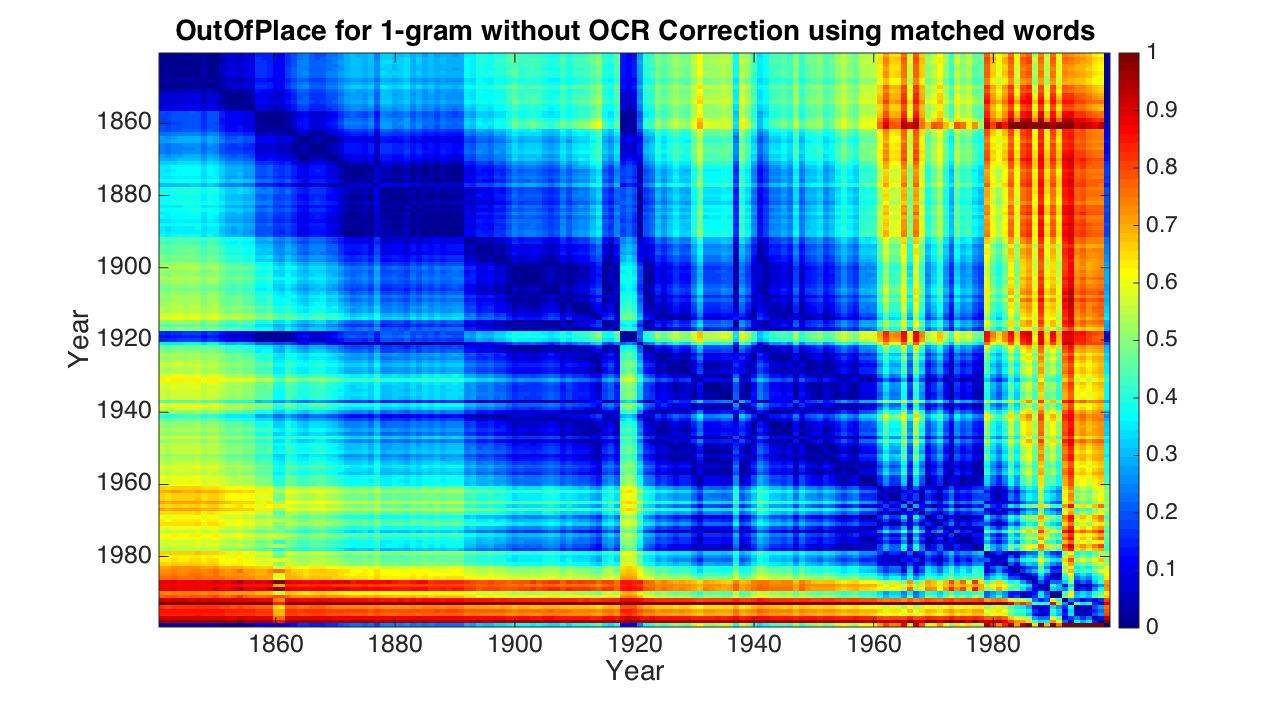
\includegraphics[scale=0.15]{Pictures/outofplace/outofplace_1-gram_noncorrectedOCR_matched_words.jpg}
        \caption{Outofplace for 1-gram without OCR correction using matched words}
        \label{outofplace_1_match_noncorrect}
    \end{minipage}\hfill
\end{figure}

\begin{figure}[H]
    \begin{minipage}[b]{0.48\linewidth}
        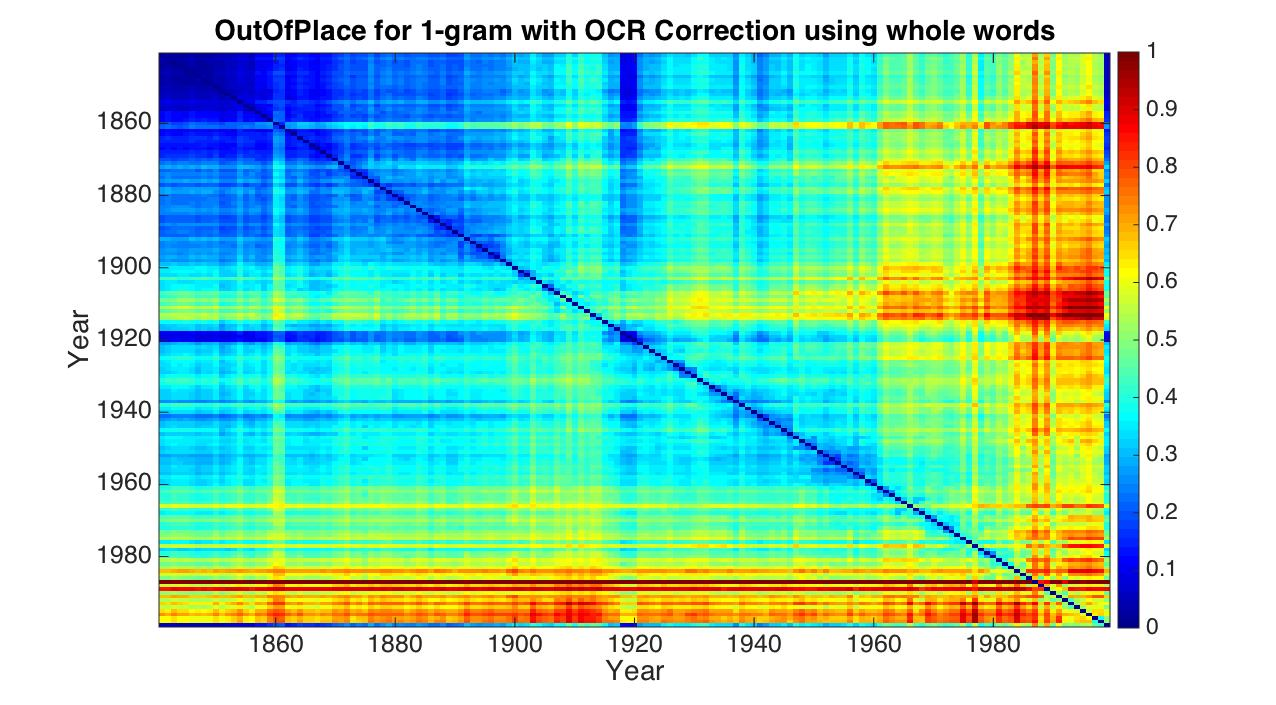
\includegraphics[scale=0.15]{Pictures/outofplace/outofplace_1-gram_correctedOCR_whole_words.jpg}
        \caption{Outofplace for 1-gram with OCR correction using whole words}
        \label{outofplace_1_all_correct}
    \end{minipage}\hfill
    \begin{minipage}[b]{0.5\linewidth}
        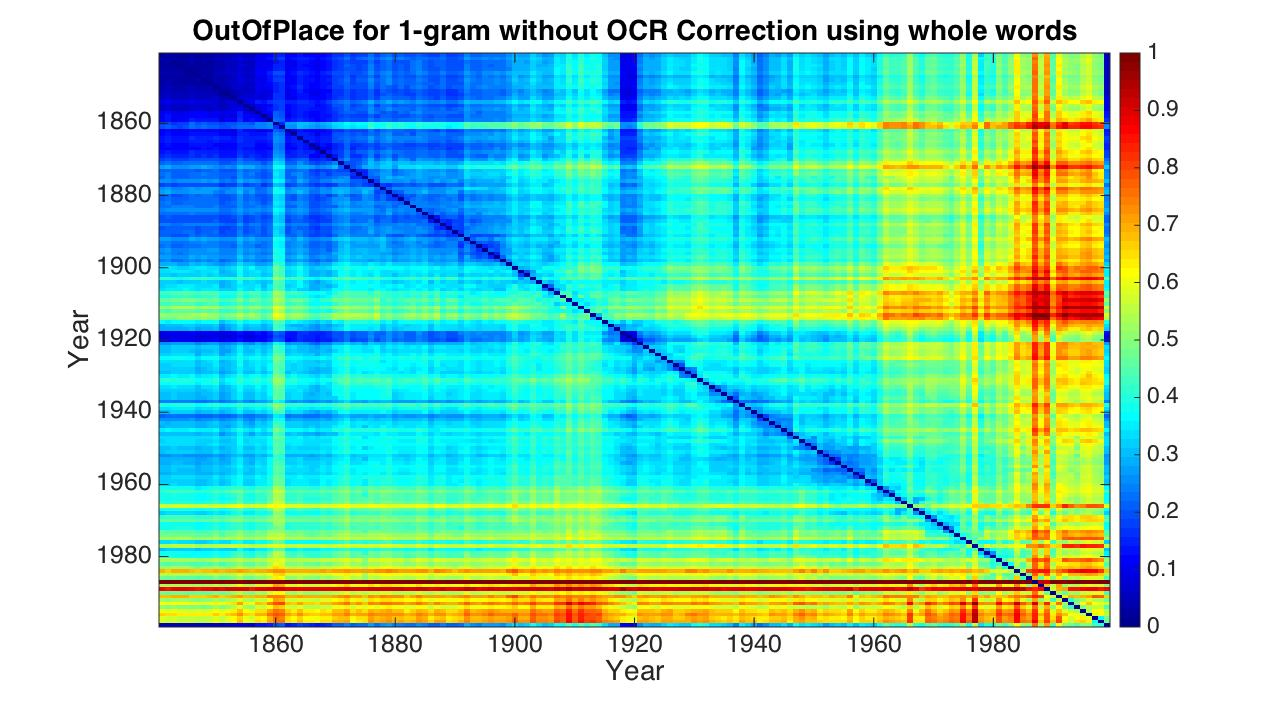
\includegraphics[scale=0.15]{Pictures/outofplace/outofplace_1-gram_noncorrectedOCR_whole_words.jpg}
        \caption{Outofplace for 1-gram without OCR correction using whole words}
        \label{outofplace_1_all_noncorrect}
    \end{minipage}\hfill
\end{figure}

\subsubsection{Analysis of results}

We can witness that for this method, the effect of OCR correction is not clear: For the same metric strategy but using different dataset (i.e., OCR corrected dataset and OCR non-corrected dataset), it has few changes in ratio but more in count (see figures \ref{outofplace_1_match_correct} and \ref{outofplace_1_match_noncorrect}; figures \ref{outofplace_1_all_correct} and \ref{outofplace_1_all_noncorrect}). More accurately, the increased count obtained by \emph{Out of Place} measurement does not affect the global picture, since most of data also increase by a similar ratio. But the feature shown by comparison is close to the description of original paper that \emph{Out of Place} provides high robustness in the face of OCR error.

However, the decision that whether we should use those unmatched words greatly impact the final distance between different years. If we only use matched words, then its result seems acceptable (see figures \ref{outofplace_1_match_correct}) where we can witness that the distance is small when comparable year is close to current year, and the distance normally increased followed by the distance between different years. But there also exists an strange phenomenon in the year $1920$ that the word appears in this year is close to the word in previous 40 to 80 years. Checking the performance of other metric in the year $1920$, we can also find a similar condition (e.g., Kullback Leibler Divergence, Chi-square). Maybe in $1920$, something happened that temporarily change the linguistic of that year. 

When it comes to the result that utilized whole words including unmatched word (see \ref{outofplace_1_all_correct}), we can witness that before year $1960$, the metric shows a good performance that closes to the rule that it ought to be. However, after year $1960$, the distance between current year and comparable year is extremely high and badly decrease the quality of this metric. We will using these two approaches in the part of dating article to find out a proper approach to fit ours dataset.

